\section{Businesses}
	\subsection{Registration}
	If you want to create a business account for \textit{Soldino} 
	visit the homepage and make sure that the slider in set on "Citizen".\\
	\begin{figure}[H]
		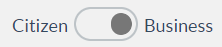
\includegraphics[width=5cm]{res/images/user_business.png}
		\centering
		\caption{Select "Business" from the slider}
	\end{figure}	
	\noindent Then, insert your business's data in the form. After you have completed 
	all the	fields with your informations press the "Sign up" button. If an 
	entry is not valid (i.e. the email address does not contain a valid 
	domain) the system will let you know and you have to correct that field 
	to continue. If all the informations are correct a pop up window will open 
	asking you to allow \textit{Soldino} to access your information.\\
	\begin{figure}[H]
		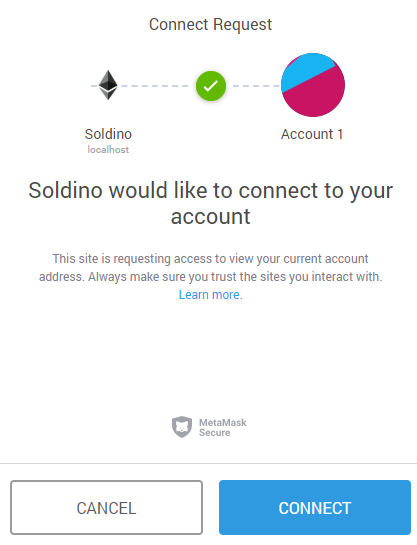
\includegraphics[width=5cm]{res/images/metamask_connect.png}
		\centering
		\caption{Connecting MetaMask to \textit{Soldino}}
	\end{figure}
	\noindent \noindent Press "Connect" and you will be redirected to a page 
	congratulating you for your registration on the platform.
	for your registration on the platform.
	\begin{figure}[H]
		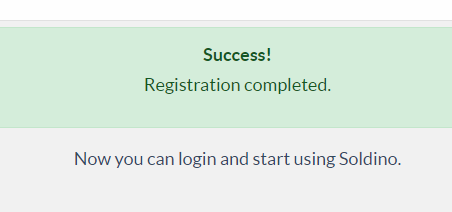
\includegraphics[width=5cm]{res/images/registration_complete.png}
		\centering
		\caption{Registration completed message}
	\end{figure}
	\subsubsection{Business is already registered}
	If your address is already registered in the platform you will see an
	error page telling you that you cannot create a new account.
	\subsection{Login}
	If you already have a business account press the "login" button on the 
	top right of the homepage. Then you will be able to buy goods and services, 
	check your orders and manage your VAT. To be able to login you have to be 
	logged in your MetaMask account.
	\subsection{Managing products}
	\subsubsection{Selling a new product}
	If you want to sell a new product you have to
	
	\subsubsection{Modifying a product}
	If you want to modify the information of a product you are selling you 
	have to 
	\subsubsection{Removing a product}
	If you want to remove a product from the platform you have to
	
	\subsection{Buying}
	\subsubsection{Searching}
	You can search for products by name using the search bar that can be found 
	right at the top of the page. After pressing enter you will be redirected to
	a page containing all results. If no matching products are found you will 
	a message showing you that.
	\subsubsection{Cart}
	After you are done searching for what you need just press the cart icon to
	go to your cart. Here you will find every item you have selected in the 
	respective quantity and above them you will see the total for your order.
	If you need to modify the quantity press the "+" or "-" buttons. \\
	When you want to proceed with the order press the "Checkout" button, 
	you will be redirected to the checkout page
	\subsubsection{Checkout}
	%PLACEHOLDER scrivere qualcosa pagina checout appena viene fatta
	\subsubsection{Past orders}
	
	\subsection{VAT management}
	If you are a business \textit{Soldino} will manage VATs for the products 
	you buy and sell on the platform automatically.
		\subsubsection{Paying VAT}
	
		\subsubsection{Deferring VAT}
		
		\subsubsection{Checking past trimesters' VAT}
		